\tikzstyle{pic}=[inner sep=0pt]
\tikzstyle{quote}=[fill=gray!30, inner sep=12pt]

\newcommand{\vogels}{
  \node[pic] (vogels) at (0, 0) {
    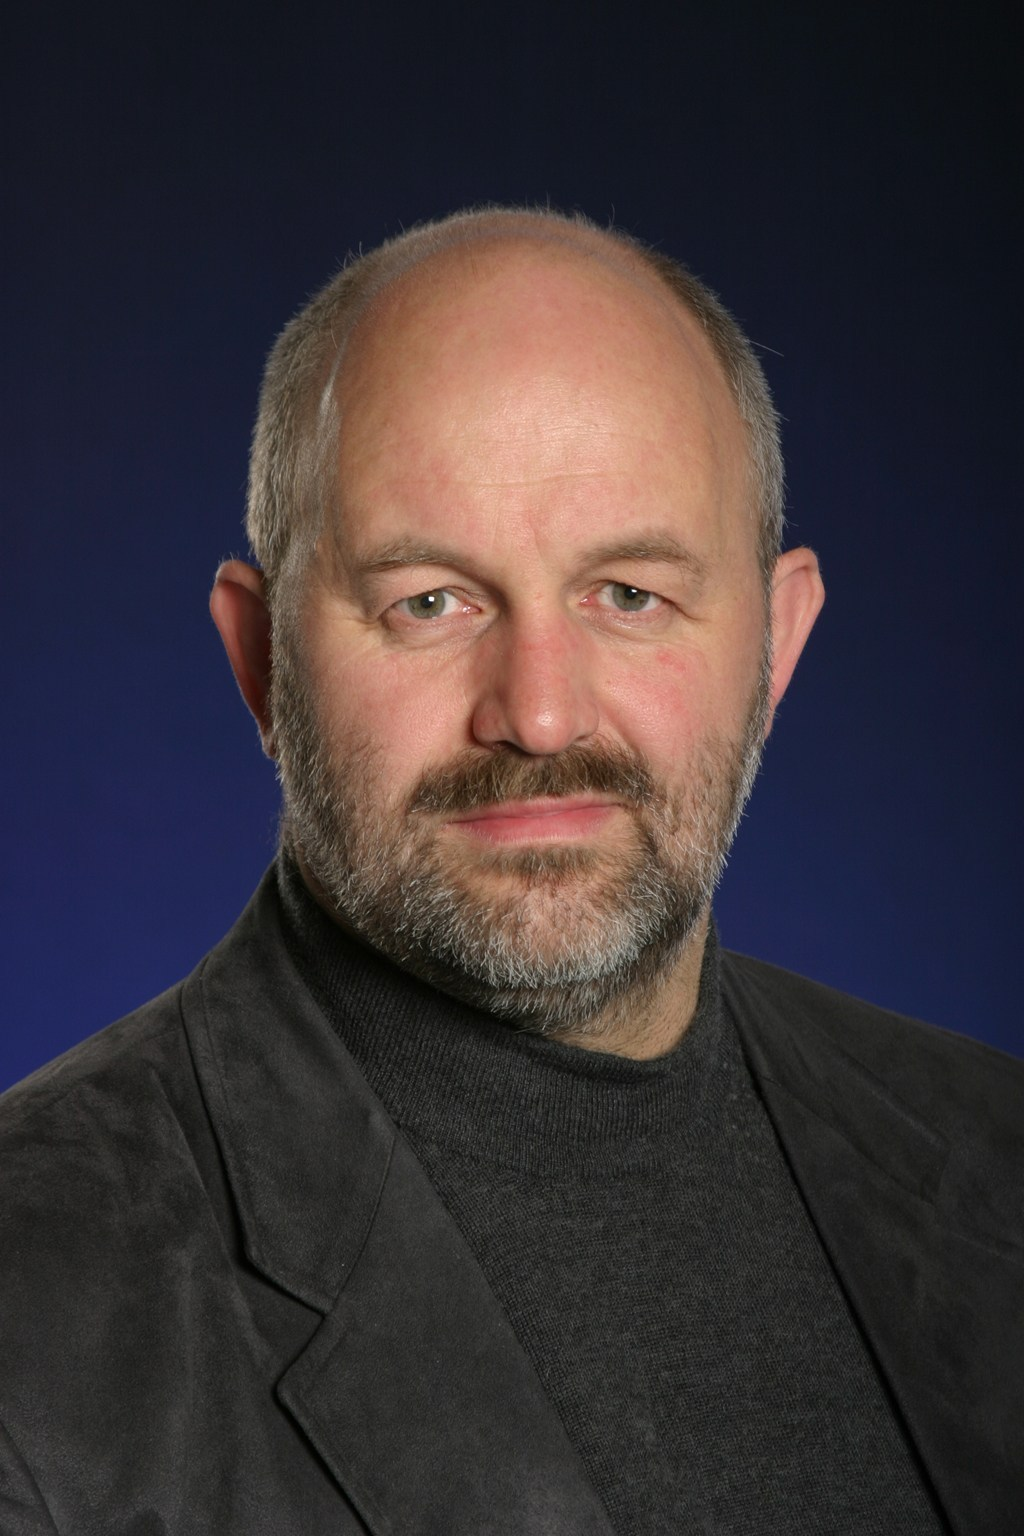
\includegraphics[
      width=0.22\textwidth,
      trim=0 75 0 25,
      clip
    ]{assets/vogels.jpg}
  };
}

\newcommand{\hoare}{
  \node[pic, right=0.2cm of vogels] (hoare) {
    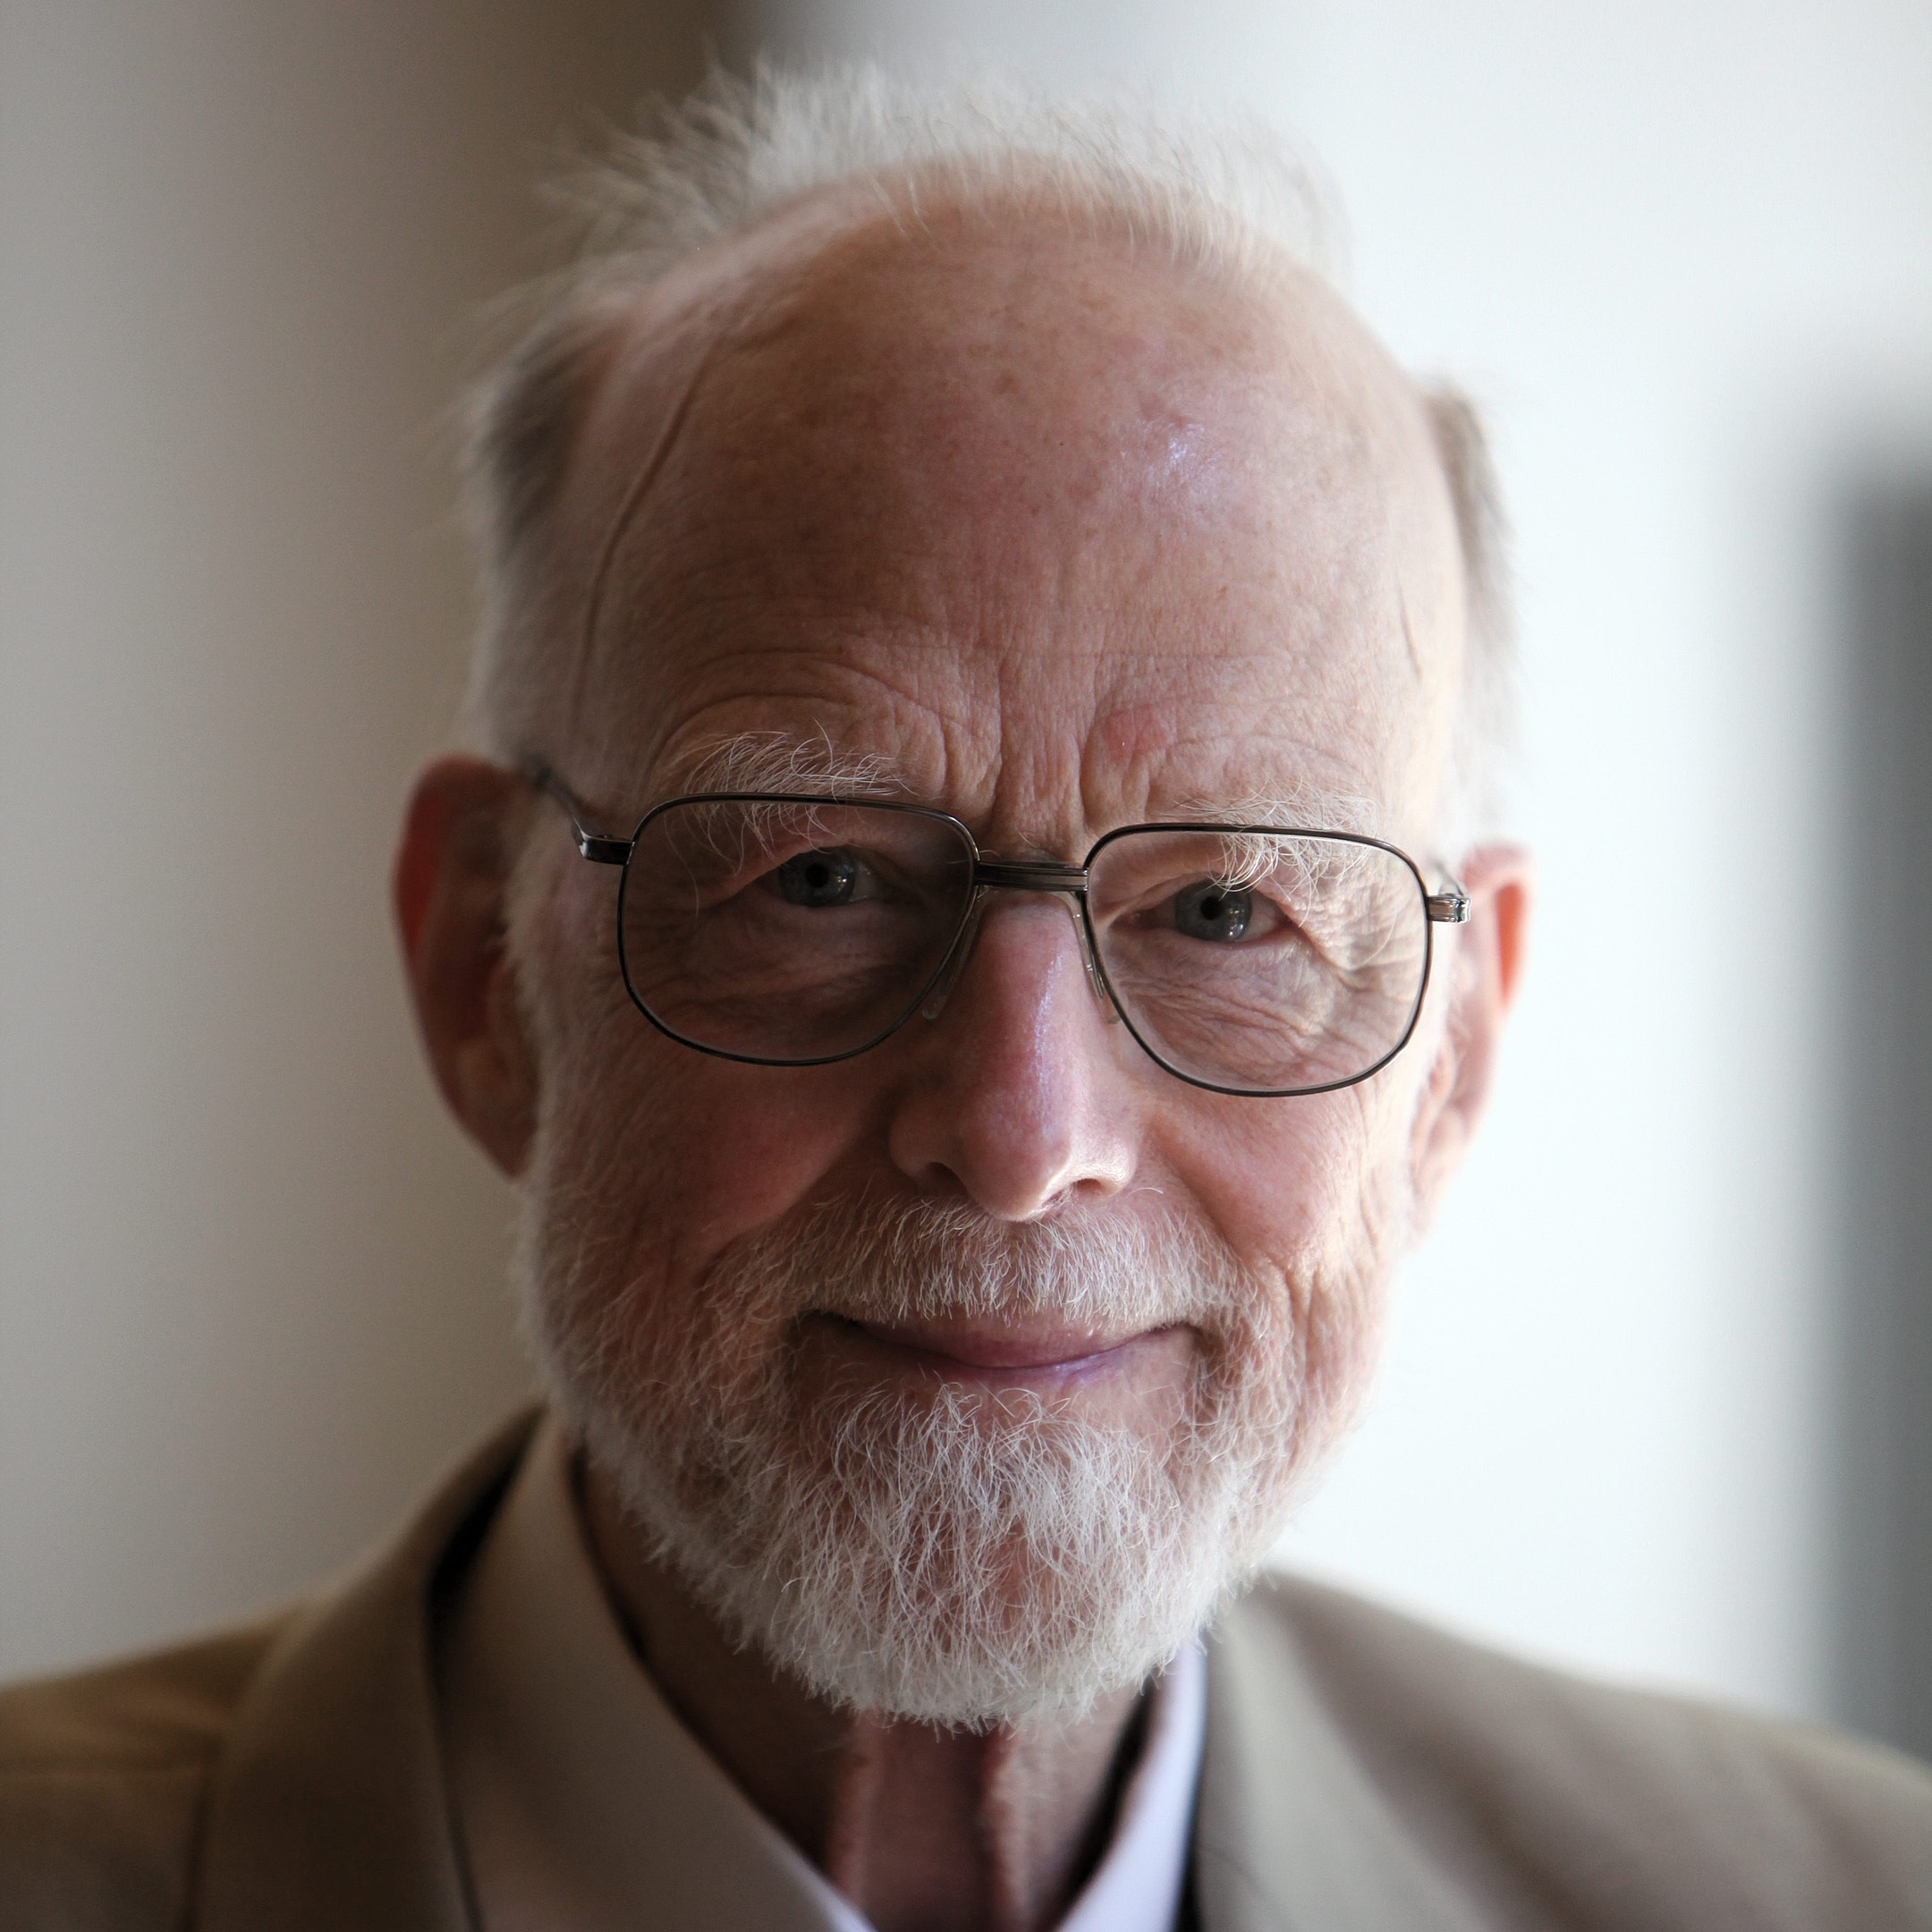
\includegraphics[width=0.22\textwidth]{assets/hoare.jpg}
  };
}

\newcommand{\lamport}{
  \node[pic, right=0.2cm of hoare] (lamport) {
    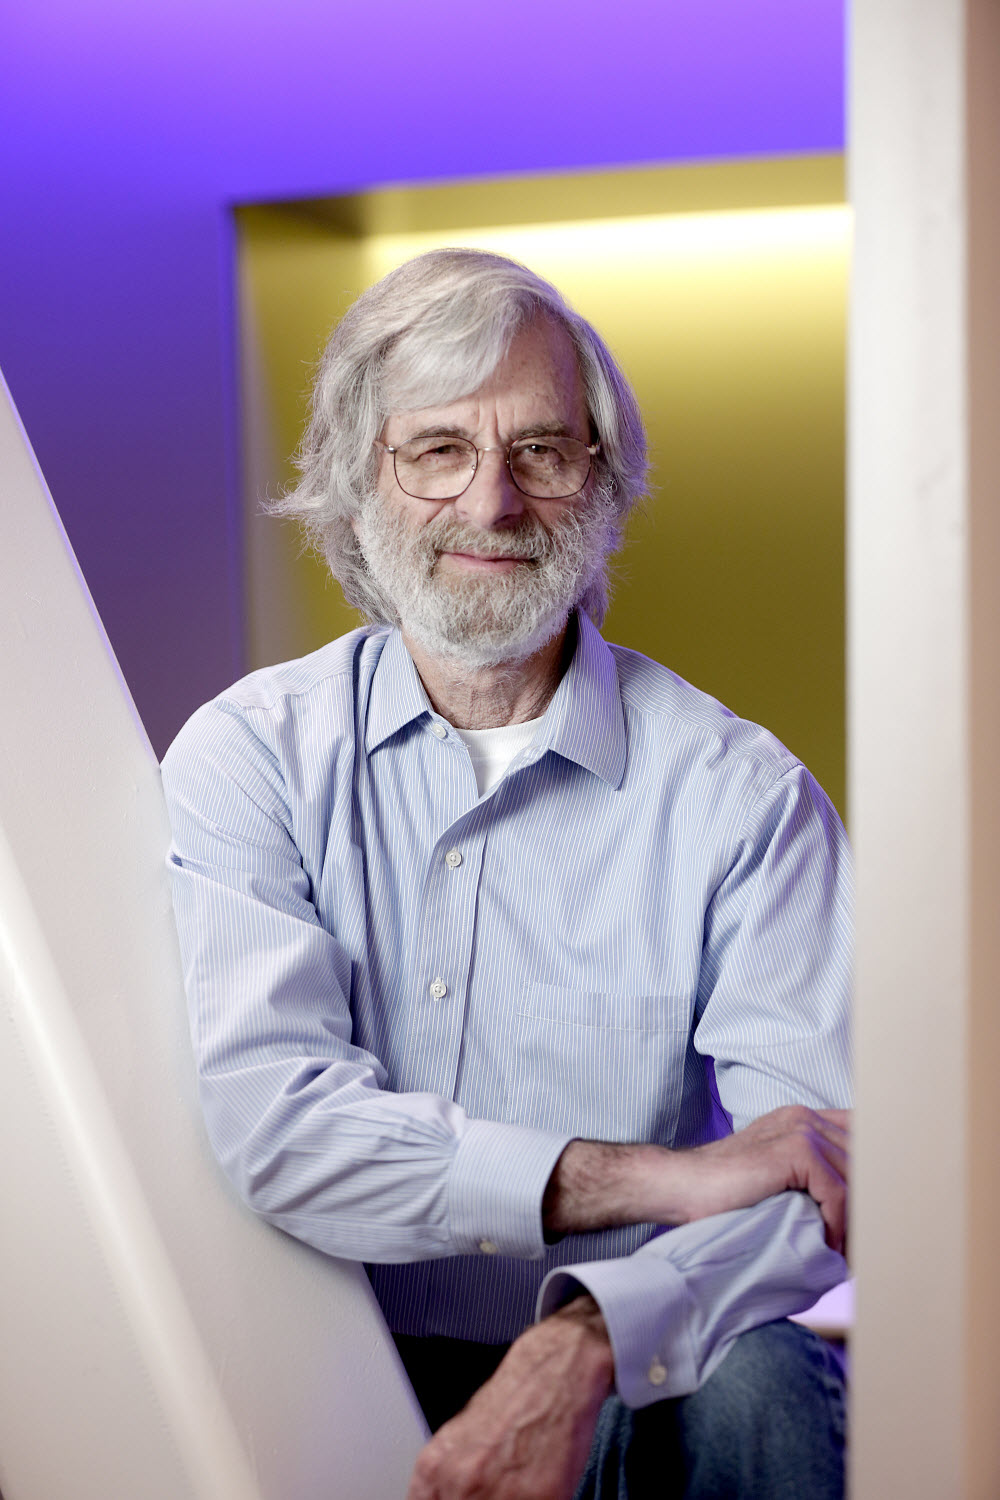
\includegraphics[
      width=0.22\textwidth,
      trim=250 700 300 200,
      clip
    ]{assets/lamport.jpg}
  };
}

\newcommand{\brewer}{
  \node[pic, right=0.2cm of lamport] (brewer) {
    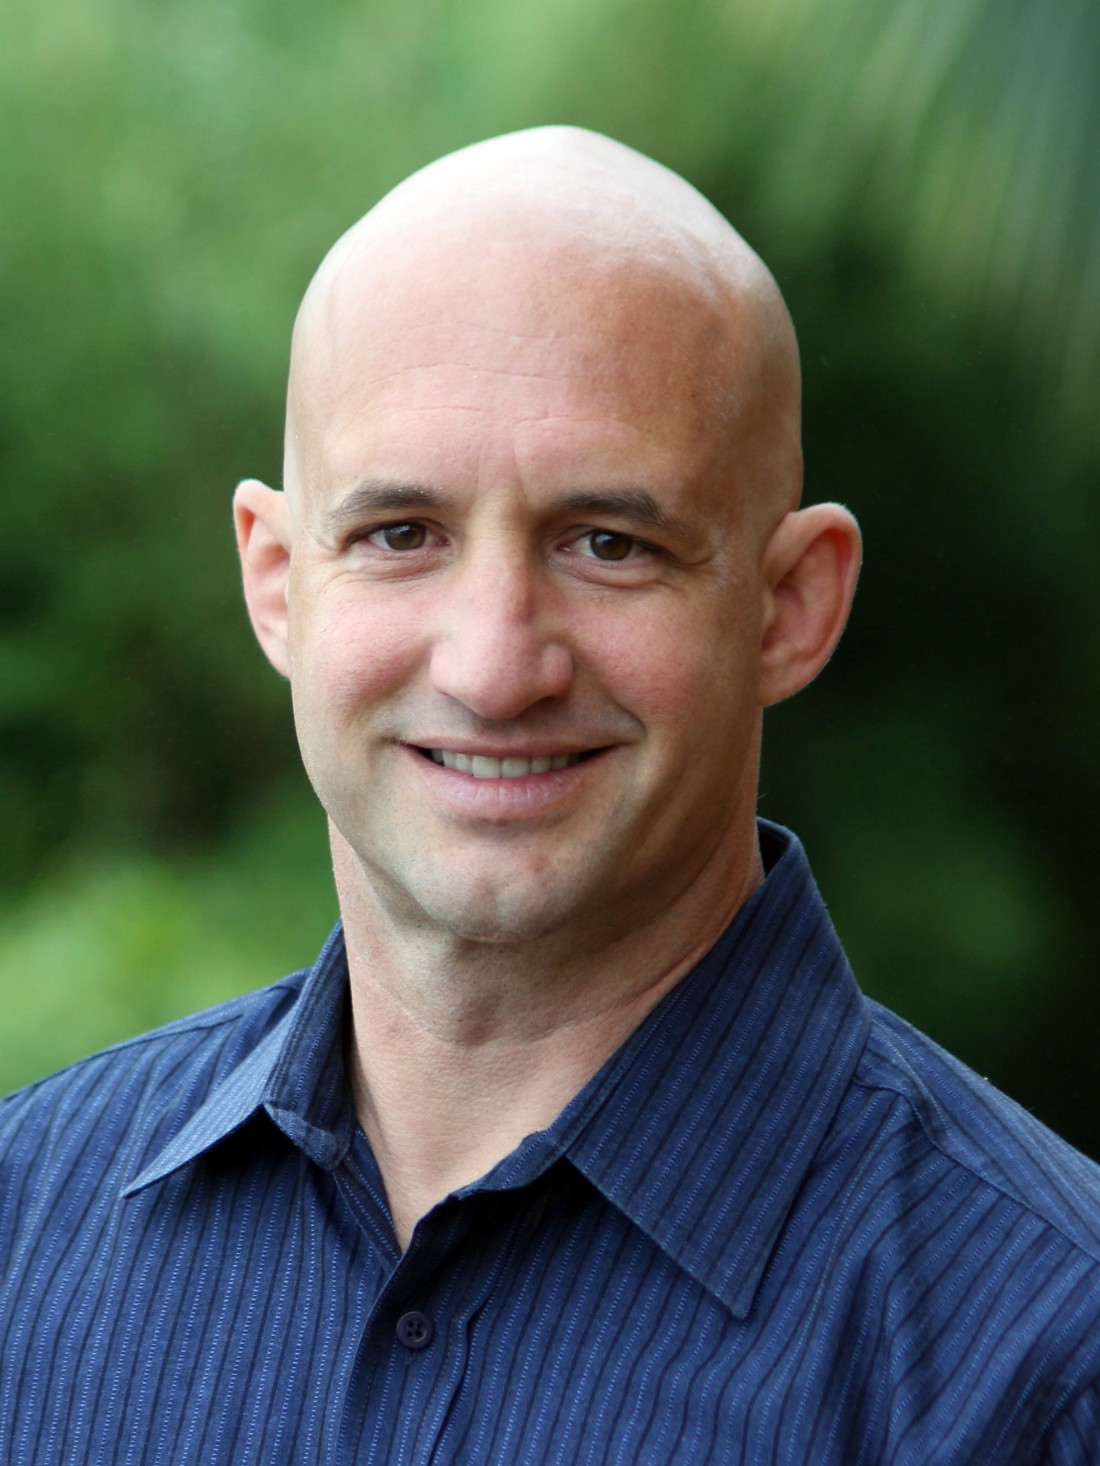
\includegraphics[
      width=0.22\textwidth,
      trim=100 300 100 100,
      clip
    ]{assets/brewer.jpg}
  };
}

\begin{frame}
  \note{%
    Hi everyone! Thanks so much for attending. I'm Michael, and today I'll be
    talking about ``Interactive Checks for Coordination Avoidance''. This is
    joint work with my advisor at UC Berkeley, Joe Hellerstein. \\[12pt]

    % I'd like to begin my talk with a short fairy tale. The fairy tale involves
    % an application developer who has some data they need to replicate.
    % Unfortunately, the application developer cannot decide whether to replicate
    % with weak consistency or strong consistency. The application developer
    % stays up all night trying to decide but eventually falls asleep at their
    % desk. In their sleep, they are visited by four wise men. And so, the fairy
    % tale begins:

    Imagine you're an application developer and you're trying to decide what
    kind of consistency you'd like to use to replicate some of your data.
  }
\end{frame}

\begin{frame}
  \begin{center}
    \begin{tikzpicture}[xscale=1.3]
      \vogels
      \node[quote, text width=0.8\textwidth, align=left] at (0, 3) {
        \Large\textit{
        Go with weak consistency. It's super duper fast and good enough for
        many applications!
        % Weak. Weak. It's weak that you're seeking.
        % \pause
        % Please learn that if you yearn your performance to peak, then turn no
        % further than weak.
      }
      };
      \path[fill=gray!30] (vogels.north) -- ++(0, 1) -- ++(0.5, 0) -- (vogels.north);
    \end{tikzpicture}
  \end{center}

  \note{%
    Someone like Werner Vogels would probably tell you to use weak consistency.
    You can implement weak consistency super duper fast, and for many
    applications, weak consistency is good enough. \\[12pt]

    % ``Weak. Weak. It's weak that you're seeking'', squeaked Werner Vogels.
    % His voice trembled, creaking, as he kept speaking.
    % ``Please learn that if you yearn your performance to peak,
    % then turn no further than weak.'' critiqued Werner.
    %
    % Werner Vogels has a good point. You can implement weak consistency super
    % duper fast, and for many applications, weak consistency is good enough.
    % But, let's continue.
  }
\end{frame}

\begin{frame}
  \begin{center}
    \begin{tikzpicture}[xscale=1.3]
      \vogels
      \hoare
      \node[quote, text width=0.8\textwidth, align=left] at (1, 3) {
        \Large\textit{
          Weakly consistent systems are so hard to reason about!
          % No. No. No more.
          % \pause
          % Weak is not easy. Weak is just treason. Please, these anomalies make
          % it so hard to reason.
        }
      };
      \path[fill=gray!30] (hoare.north) -- ++(0, 1) -- ++(0.5, 0) -- (hoare.north);
    \end{tikzpicture}
  \end{center}

  \note{%
    Tony Hoare would encourage us not to settle for weak consistency because a
    weakly consistent system is hard to reason about.

    % ``No, no, no more'' groaned Tony Hoare.
    % He moaned, he lamented, his soul was tormented
    % ``Weak is not easy. Weak is just treason.
    % Please, these anomalies, make it so hard to reason.''
    %
    % You see, Tony Hoare encourages us not to settle for weak consistency
    % because a weakly consistent system is very hard to reason about.
  }
\end{frame}

\begin{frame}
  \begin{center}
    \begin{tikzpicture}[xscale=1.3]
      \vogels
      \hoare
      \lamport
      \node[quote, text width=0.8\textwidth, align=left] at (2, 3) {
        \Large\textit{
          Go with a strongly consistent system! I think there are some good
          algorithms for that kind of stuff.
          % You see, I agree.
          % \pause
          % Weak is just wrong, not right for long. To defend your end users, you
          % must go with strong.
        }
      };
      \path[fill=gray!30] (lamport.north) -- ++(0, 0.5) -- ++(0.25, 0) -- (lamport.north);
    \end{tikzpicture}
  \end{center}

  \note{%
    Leslie Lamport would agree. He would encourage us to choose strong
    consistency. Strongly consistent systems are much easier to reason about.

    % ``You see, I agree'', says he, the ever mesmerizing Leslie.
    % ``Weak is just wrong, not right for long.
    % To defend your end users, you must go with strong.''
    %
    % Leslie Lamport encourages us to choose strong consistency becausesStrongly
    % consistent systems are much easier to reason about. After all a strongly
    % consistent system to end users looks exactly like a system that's not even
    % distributed.
  }
\end{frame}

\begin{frame}
  \begin{center}
    \begin{tikzpicture}[xscale=1.3]
      \vogels
      \hoare
      \lamport
      \brewer
      \node[quote, text width=0.8\textwidth, align=left] at (3, 3) {
        \Large\textit{
          Not so fast!
          % Alas, not so fast!
          % \pause
          % Consistency weak but not weary, strong but not nearly as fast as you
          % think when you hear my CAP theory.
        }
      };
      \path[fill=gray!30] (brewer.north) -- ++(0, 1) -- ++(-1, 0) -- (brewer.north);
    \end{tikzpicture}
  \end{center}

  \note{%
    Eric Brewer would counter that strong consistency isn't perfect. Strong
    consistency comes at the price of availability and performance. So we're in
    a bit of a pickle. Weak consistency is too confusing and strong consistency
    is too heavy handed.

    %
    % ``Alas, not so fast'', Brewer the dapper chap clapped back.
    % ``Consistency weak but not weary, strong but not nearly
    % as fast as you think when you hear my CAP theory.''
    %
    % Eric Brewer is right. Surely, strong consistency comes at the price of
    % availability and performance. So our application developer is in a bit of a
    % pickle. Weak consistency is too confusing and strong consistency is too
    % heavy handed. Fortunately, a hero emerges to save the day.
  }
\end{frame}

\begin{frame}
  \begin{center}
    \begin{tikzpicture}[xscale=1.3]
      \node[pic] (bailis) at (0, 0) {
\includegraphics[width=0.25\textwidth]{assets/bailis.jpg}};
      \node[quote, text width=0.8\textwidth, align=left] at (0, 3) {
        \Large\textit{Why not have both?}
      };
      \path[fill=gray!30] (bailis.north) -- ++(0, 1.5) -- ++(1, 0) -- (bailis.north);
    \end{tikzpicture}
  \end{center}

  \note{%
    % Out teetered Peter, with swagger demeanor.
    % ``Why not have both?'' quoth the Peter.
    % The end.

    Fortunately, Peter Bailis can save the and reminding us of when in 2014, he
    and some other smart folks including Alan defined invariant confluence as a
    way to get the benefits of both weak and strong consistency.

    Invariant confluence will be the topic of this talk, so let's build some
    intuition on what invariant confluence is.
  }
\end{frame}
